% Compile with XeLaTeX or LuaLaTeX
\documentclass[12pt,a4paper]{article}

\usepackage[a4paper,margin=2.5cm]{geometry}
\usepackage{fontspec}
\usepackage{polyglossia}
\usepackage{xcolor}
\usepackage{graphicx}
\usepackage{booktabs}
\usepackage{changepage}
\usepackage{float}
\usepackage{pdflscape}
\usepackage{amsmath}

\setmainlanguage{greek}
\setotherlanguage{english}
\setmainfont{DejaVu Sans}
\setsansfont{DejaVu Sans}
\setmonofont{DejaVu Sans Mono}
\newfontfamily\greekfont[Script=Greek]{DejaVu Sans}
\newfontfamily\greekfontsf[Script=Greek]{DejaVu Sans}
\newfontfamily\greekfonttt[Script=Greek]{DejaVu Sans Mono}

\definecolor{wordblue}{RGB}{0,112,192}

\pagestyle{empty}
\setlength{\parindent}{0pt}

\begin{document}

\vspace*{0.5cm}

\begin{adjustwidth}{1.5cm}{1.5cm}

{\centering\itshape\fontsize{14}{16}\selectfont
Δομή αρχείου ελέγχου ενεργειών εργασίας μαθήματος Κλιματισμού\par}

\vspace{0.5cm}

{\fontsize{12}{14}\selectfont
Στοιχεία φοιτητή / φοιτητών:\par}

\vspace{0.15cm}

{\fontsize{12}{14}\selectfont
Ρακοβαλής Παύλος, Α.Ε.Μ. 6931\par}

\vspace{0.55cm}

{\color{wordblue}\bfseries\fontsize{13}{15}\selectfont
Βήμα 1. Αποτύπωση βασικών στοιχείων κτιρίου\par}

\vspace{0.3cm}

{\bfseries 1α. Επιφάνεια Κτιρίου\par}

\vspace{0.1cm}

{\bfseries\fontsize{13}{15}\selectfont
145.00 m²\par}

\vspace{0.35cm}

{\bfseries 1β. Κάτοψη Κτιρίου\par}

\vspace{0.2cm}

\begin{center}
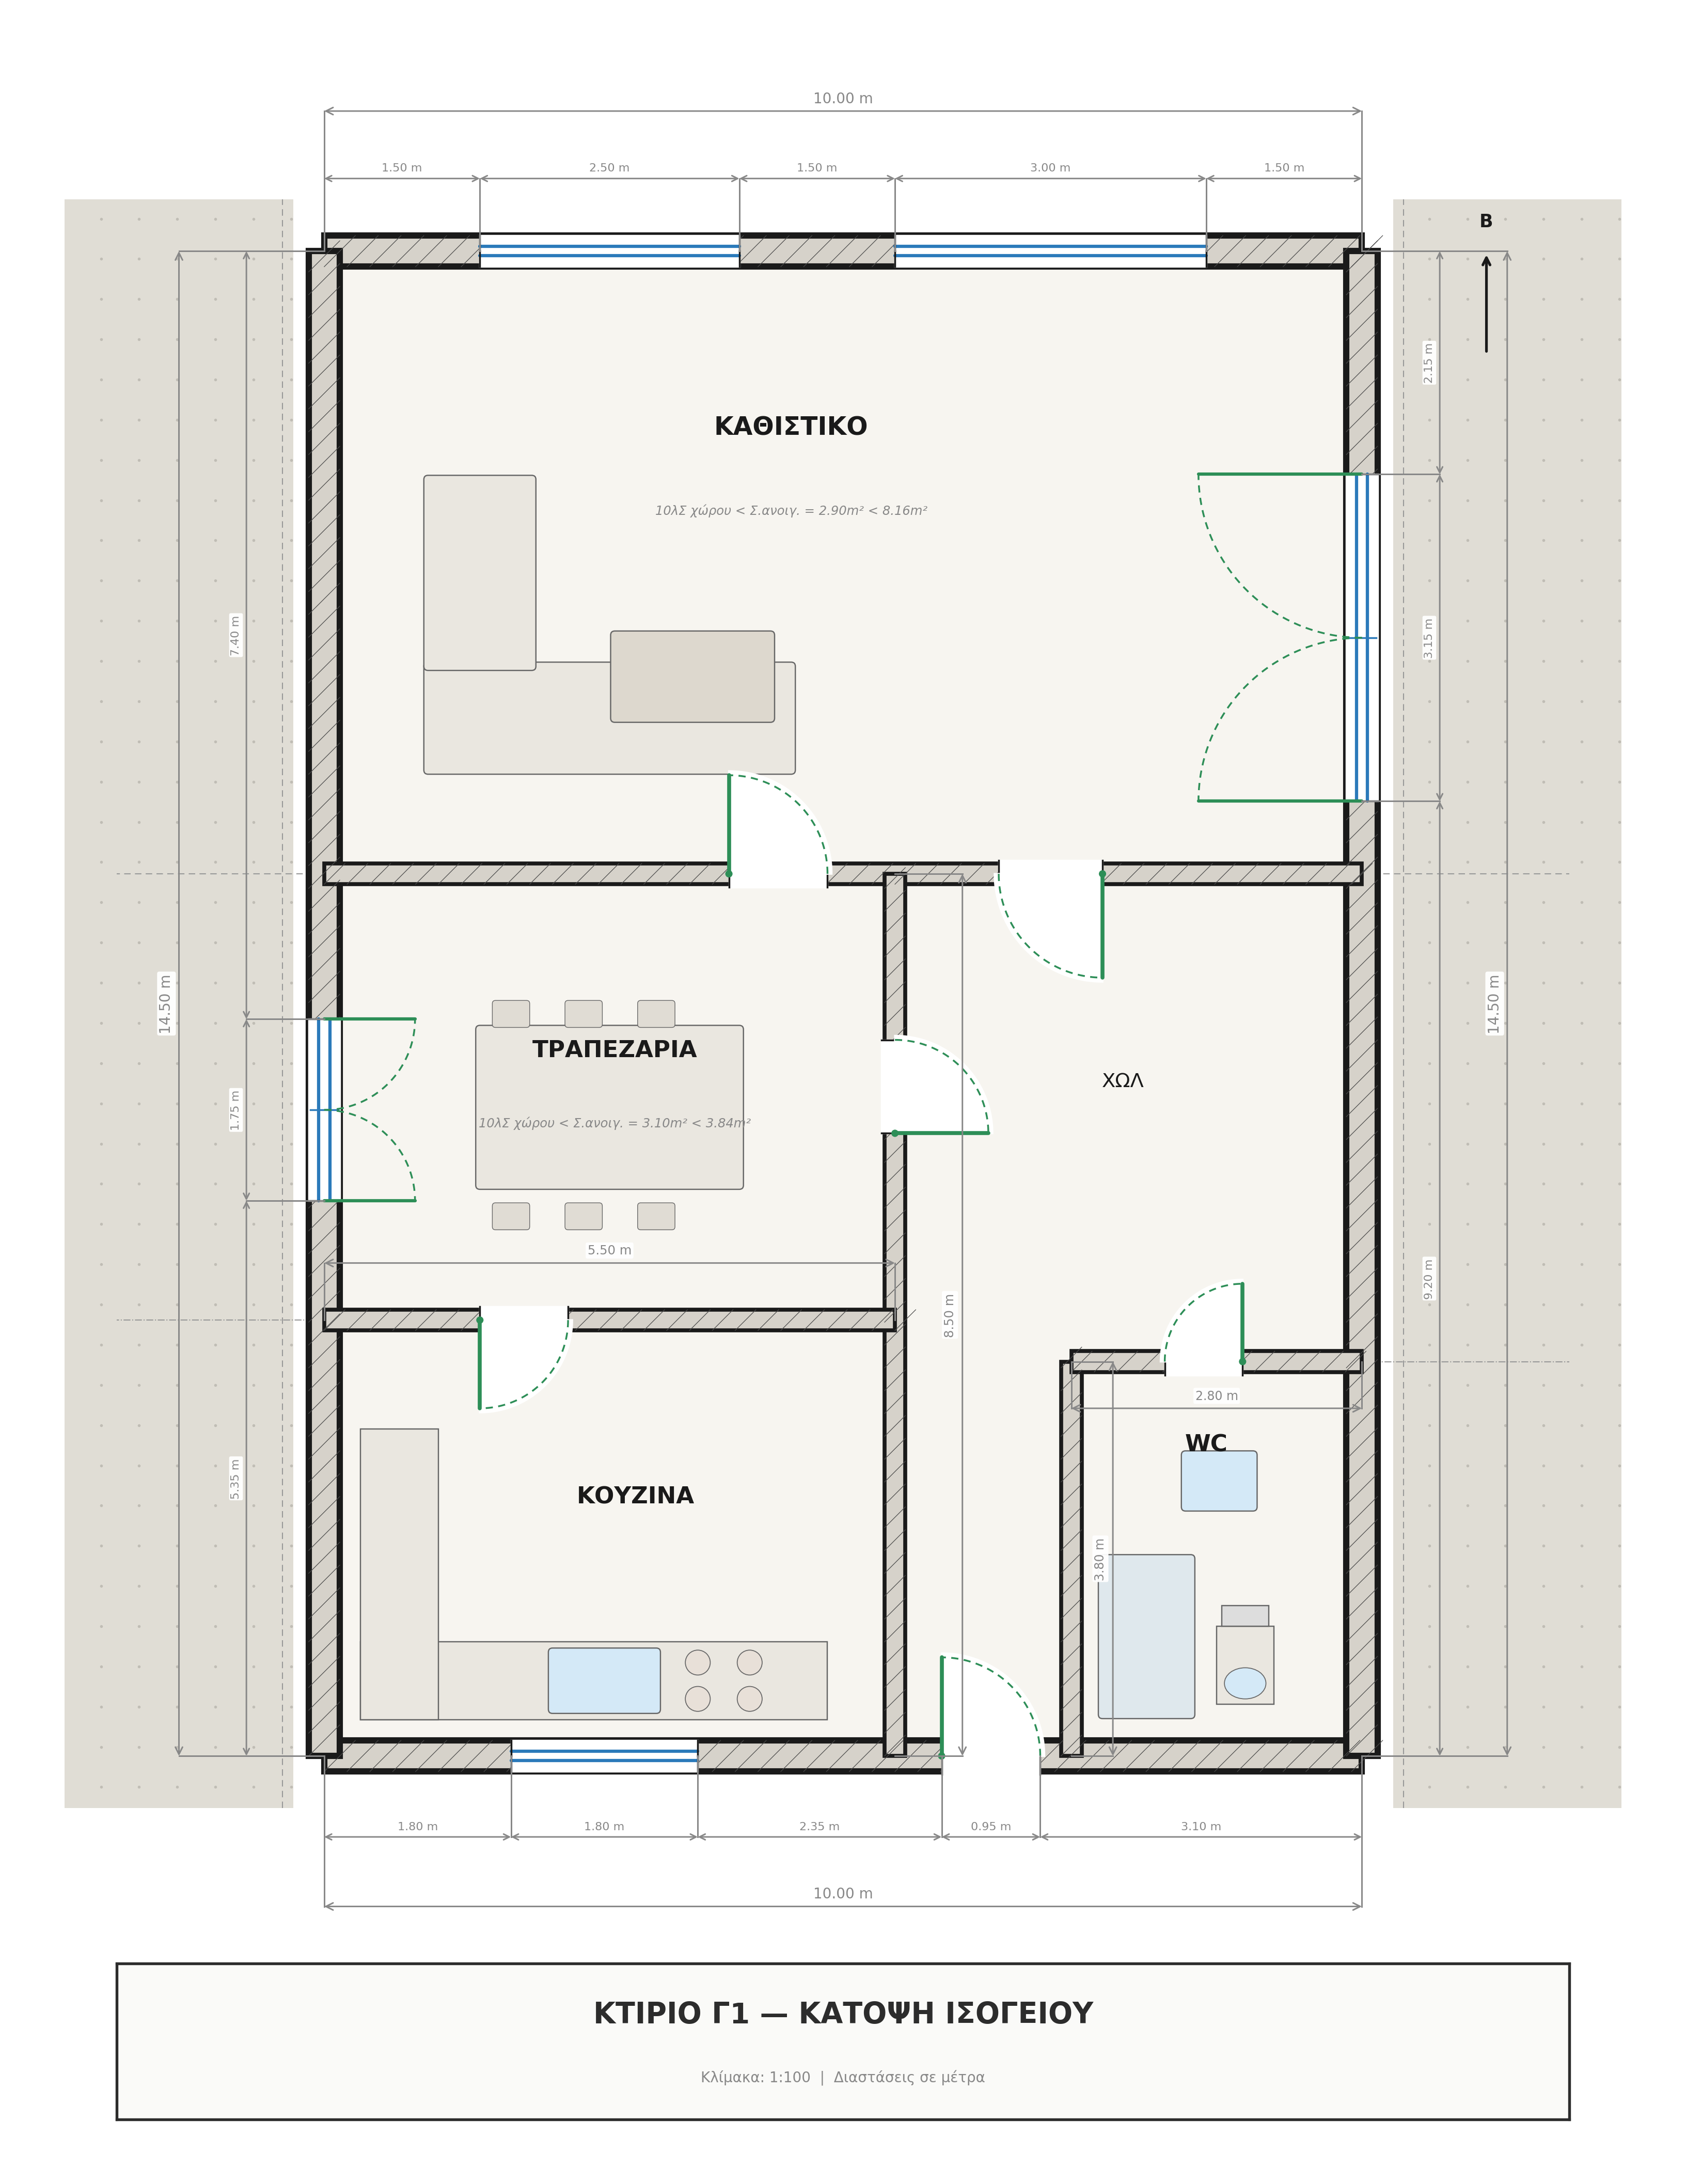
\includegraphics[width=0.82\linewidth]{floor_plan_G1.png}
\end{center}

\end{adjustwidth}

\clearpage

\begin{adjustwidth}{1.5cm}{1.5cm}

{\bfseries 1γ. Πίνακας Δομικών Στοιχείων (διαφ. 5 οδηγού)\par}

\vspace{0.2cm}

{\fontsize{12}{14}\selectfont
Ο σχετικός πίνακας παρατίθεται αναλυτικά στο Βήμα 2 που ακολουθεί.\par}

\vspace{0.55cm}

{\color{wordblue}\bfseries\fontsize{13}{15}\selectfont
Βήμα 2. Προσδιορισμός συντελεστή θερμοπερατότητας στοιχείων\par}

\vspace{0.3cm}

{\fontsize{12}{14}\selectfont
Θα συμπληρωθεί στον πίνακα 1γ.\par}

\end{adjustwidth}

\setcounter{table}{5}
\begin{landscape}
\begin{table}[H]
\centering
\renewcommand{\arraystretch}{1.3}
\footnotesize
\caption{Βήμα 1α -- Καταγραφή δομικών στοιχείων εξωτερικού περιβλήματος}
\begin{tabular}{p{1.9cm}p{3.0cm}p{4.0cm}p{2.3cm}p{2.2cm}p{1.5cm}p{1.8cm}p{1.7cm}p{2.0cm}}
\toprule
\textbf{Συμβο\-λι\-σμός} & \textbf{Τύπος στοιχείου} & \textbf{Υλικά κατα\-σκευής} & \textbf{Προσανα\-τολι\-σμός} & \textbf{Μήκος/ πλάτος (m)} & \textbf{Ύψος (m)} & \textbf{Επι\-φάνεια (\(\mathrm{m^2}\))} & \textbf{Αριθμός επι\-φα\-νειών} & \textbf{Συντ. θερμο\-περα\-τότητας \(\mathrm{W/(m^2K)}\)} \\
\midrule
\multicolumn{9}{l}{\textbf{Αδιαφανή στοιχεία}} \\
\midrule
\(W_{L\mathrm{B}}\) & Εξωτερικός τοίχος & Τούβλο / μόνωση / σκυρόδεμα / επίχρισμα & Βορράς (Β) & 10.00 & 3.00 & 22.30 & 1 & 0.45 \\
\(W_{L\mathrm{N}}\) & Εξωτερικός τοίχος & Τούβλο / μόνωση / σκυρόδεμα / επίχρισμα & Νότος (Ν) & 10.00 & 3.00 & 27.48 & 1 & 0.45 \\
\(W_{L\mathrm{A}}\) & Εξωτερικός τοίχος & Τούβλο / μόνωση / σκυρόδεμα / επίχρισμα & Ανατολή (Α) & 14.50 & 3.00 & 35.94 & 1 & 0.45 \\
\(W_{L\Delta}\) & Εξωτερικός τοίχος & Τούβλο / μόνωση / σκυρόδεμα / επίχρισμα & Δύση (Δ) & 14.50 & 3.00 & 39.30 & 1 & 0.45 \\
\(R\) & Οροφή -- επαφή με εξωτερικό αέρα & Ο.Σ. / μόνωση / ασφαλτική επικάλυψη & -- & 10.00 \(\times\) 14.50 & -- & 145.00 & 1 & 0.40 \\
\(F\) & Δάπεδο -- επαφή με το έδαφος & Ο.Σ. / μόνωση / πλακάκι & -- & 10.00 \(\times\) 14.50 & -- & 145.00 & 1 & 0.60 \\
\midrule
\multicolumn{9}{l}{\textbf{Διαφανή στοιχεία}} \\
\midrule
\(W_{i\mathrm{B}1}\) & Παράθυρο -- καθιστικό & Αλουμίνιο / διπλό τζάμι & Βορράς (Β) & 2.50 & 1.40 & 3.50 & 1 & 2.40 \\
\(W_{i\mathrm{B}2}\) & Παράθυρο -- καθιστικό & Αλουμίνιο / διπλό τζάμι & Βορράς (Β) & 3.00 & 1.40 & 4.20 & 1 & 2.40 \\
\(W_{i\mathrm{N}}\) & Παράθυρο -- κουζίνα & Αλουμίνιο / διπλό τζάμι & Νότος (Ν) & 1.80 & 1.40 & 2.52 & 1 & 2.40 \\
\(W_{i\mathrm{A}}\) & Μπαλκονόπορτα (δίφυλλη) -- καθιστικό & Αλουμίνιο / διπλό τζάμι & Ανατολή (Α) & 3.15 & 2.40 & 7.56 & 1 & 2.40 \\
\(W_{i\Delta}\) & Μπαλκονόπορτα (δίφυλλη) -- τραπεζαρία & Αλουμίνιο / διπλό τζάμι & Δύση (Δ) & 1.75 & 2.40 & 4.20 & 1 & 2.40 \\
\midrule
\multicolumn{6}{r}{\textbf{Σύνολο αδιαφανών επιφανειών}} & \textbf{415.02} & \multicolumn{2}{l}{} \\
\multicolumn{6}{r}{\textbf{Σύνολο διαφανών επιφανειών}} & \textbf{21.98} & \multicolumn{2}{l}{} \\
\bottomrule
\end{tabular}
\end{table}
\end{landscape}

\begin{adjustwidth}{1.5cm}{1.5cm}
{\color{wordblue}\bfseries\fontsize{13}{15}\selectfont
Βήμα 3. Υπολογισμός φορτίων ψύξης με τη μέθοδο \textenglish{CLTD}\par}

\vspace{0.3cm}

{\fontsize{12}{14}\selectfont
Παρατίθενται οι Πίνακες 28 και 29 του report με το συμπληρωμένο φύλλο εργασίας
\textenglish{CLTD} για τα αισθητά, λανθάνοντα και συνολικά ψυκτικά φορτία.\par}
\end{adjustwidth}

\setcounter{table}{27}
\begin{landscape}
\begin{table}[H]
\centering
\renewcommand{\arraystretch}{1.35}
\scriptsize
\caption{Συμπληρωμένο φύλλο εργασίας \textenglish{CLTD} -- αισθητά φορτία}
\resizebox{\linewidth}{!}{%
\begin{tabular}{llcc*{5}{cc}}
\toprule
\textbf{Στοιχείο} & \textbf{Τύπος / σχόλιο} & \textbf{U} & \textbf{A} &
\multicolumn{2}{c}{\textbf{08:00}} &
\multicolumn{2}{c}{\textbf{12:00}} &
\multicolumn{2}{c}{\textbf{16:00}} &
\multicolumn{2}{c}{\textbf{20:00}} &
\multicolumn{2}{c}{\textbf{24:00}} \\
\cmidrule(lr){5-6}\cmidrule(lr){7-8}\cmidrule(lr){9-10}\cmidrule(lr){11-12}\cmidrule(lr){13-14}
\textbf{} & \textbf{} & \(\mathbf{\mathrm{W/(m^2K)}}\) & \(\mathbf{\mathrm{m^2}}\) &
\textbf{CLTD/CLF} & \textbf{\(q\) [W]} &
\textbf{CLTD/CLF} & \textbf{\(q\) [W]} &
\textbf{CLTD/CLF} & \textbf{\(q\) [W]} &
\textbf{CLTD/CLF} & \textbf{\(q\) [W]} &
\textbf{CLTD/CLF} & \textbf{\(q\) [W]} \\
\midrule
\multicolumn{14}{l}{\textbf{Τοίχοι -- \(q = U \cdot A \cdot CLTD_{\mathrm{corr}}\), με \(CLTD_{\mathrm{corr}}=(CLTD+LM)\cdot K+0.6\)}} \\
Τοίχος Βορράς & Ομάδα D / \(K=0.65\) & 0.45 & 22.30 & 2.8 & 24.3 & 5.0 & 38.6 & 5.6 & 42.5 & 5.6 & 42.5 & 4.4 & 34.7 \\
Τοίχος Νότος & Ομάδα D / \(K=0.65\) & 0.45 & 27.48 & 3.3 & 33.9 & 9.4 & 83.0 & 8.3 & 74.1 & 6.1 & 56.5 & 5.0 & 47.6 \\
Τοίχος Ανατολή & Ομάδα D / \(K=0.65\) & 0.45 & 35.94 & 12.8 & 144.3 & 11.7 & 132.7 & 7.8 & 91.7 & 6.1 & 73.8 & 5.6 & 68.6 \\
Τοίχος Δύση & Ομάδα D / \(K=0.65\) & 0.45 & 39.30 & 3.3 & 48.5 & 3.3 & 48.5 & 12.2 & 150.9 & 13.3 & 163.5 & 10.0 & 125.6 \\
\textbf{Σύνολο τοίχων} &  &  &  &  & \textbf{251.0} &  & \textbf{302.9} &  & \textbf{359.2} &  & \textbf{336.3} &  & \textbf{276.5} \\
\midrule
\multicolumn{14}{l}{\textbf{Οροφή -- \(q = U \cdot A \cdot CLTD_{\mathrm{corr}} \cdot f\), με \(CLTD_{\mathrm{corr}}=(CLTD+0.5)\cdot 1.0+0.6\)}} \\
Οροφή & Τύπος 9 / \(K=1.0\) / \(f=1.0\) & 0.40 & 145.00 & 2.2 & 191.4 & 8.3 & 545.2 & 15.6 & 968.6 & 15.0 & 933.8 & 8.9 & 580.0 \\
\midrule
\multicolumn{14}{l}{\textbf{Υαλοπίνακες λόγω αγωγής -- \(q = U \cdot A \cdot (CLTD+0.6)\)}} \\
Π1+Π2 Βορράς & Διπλός υαλοπίνακας & 2.40 & 7.70 & 0 & 11.1 & 5 & 103.5 & 8 & 158.9 & 4 & 85.0 & 1 & 29.6 \\
Π3 Νότος & Διπλός υαλοπίνακας & 2.40 & 2.52 & 0 & 3.6 & 5 & 33.9 & 8 & 52.0 & 4 & 27.8 & 1 & 9.7 \\
Μπαλκονόπορτα Ανατολή & Διπλός υαλοπίνακας & 2.40 & 7.56 & 0 & 10.9 & 5 & 101.6 & 8 & 156.0 & 4 & 83.5 & 1 & 29.0 \\
Μπαλκονόπορτα Δύση & Διπλός υαλοπίνακας & 2.40 & 4.20 & 0 & 6.0 & 5 & 56.4 & 8 & 86.7 & 4 & 46.4 & 1 & 16.1 \\
\textbf{Σύνολο αγωγ. ανοιγμάτων} &  &  &  &  & \textbf{31.7} &  & \textbf{295.4} &  & \textbf{453.7} &  & \textbf{242.7} &  & \textbf{84.4} \\
\midrule
\multicolumn{14}{l}{\textbf{Ηλιακά κέρδη ανοιγμάτων -- \(q = A \cdot SC \cdot SHGF_{\max} \cdot CLF\)}} \\
Π1+Π2 Βορράς & \(SC=0.69,\; SHGF_{\max}=131\) & -- & 7.70 & 0.65 & 452.4 & 0.89 & 619.4 & 0.75 & 522.0 & 0.18 & 125.3 & 0.10 & 69.6 \\
Π3 Νότος & \(SC=0.69,\; SHGF_{\max}=190\) & -- & 2.52 & 0.23 & 76.0 & 0.83 & 274.2 & 0.35 & 115.6 & 0.09 & 29.7 & 0.05 & 16.5 \\
Μπαλκονόπορτα Ανατολή & \(SC=0.69,\; SHGF_{\max}=527\) & -- & 7.56 & 0.80 & 2199.2 & 0.27 & 742.2 & 0.17 & 467.3 & 0.05 & 137.5 & 0.03 & 82.5 \\
Μπαλκονόπορτα Δύση & \(SC=0.69,\; SHGF_{\max}=527\) & -- & 4.20 & 0.11 & 168.0 & 0.17 & 259.6 & 0.82 & 1252.3 & 0.12 & 183.3 & 0.06 & 91.6 \\
\textbf{Σύνολο ηλιακών κερδών} &  &  &  &  & \textbf{2895.6} &  & \textbf{1895.5} &  & \textbf{2357.3} &  & \textbf{475.7} &  & \textbf{260.2} \\
\midrule
\multicolumn{14}{l}{\textbf{Αερισμός / διείσδυση -- \(q_{\mathrm{sens}} = \dot{m} \cdot C_p \cdot \Delta T\), με \(ACH=0.5\), \(\dot{m}=0.0727\,\mathrm{kg/s}\)}} \\
Αερισμός & \(T_o=26.8,\; \Delta T=0.8\) έως \(T_o=27.0,\; \Delta T=1.0\) & -- & -- & -- & 56.8 & -- & 558.7 & -- & 723.2 & -- & 361.2 & -- & 73.3 \\
\midrule
\multicolumn{14}{l}{\textbf{Εσωτερικά χωρίσματα -- ενιαία ζώνη, \(q=0\)}} \\
Εσωτερικά χωρίσματα & \(\Delta T = 0\) & -- & -- & -- & 0.0 & -- & 0.0 & -- & 0.0 & -- & 0.0 & -- & 0.0 \\
\midrule
\multicolumn{14}{l}{\textbf{Εσωτερικά αισθητά φορτία}} \\
Άνθρωποι & \(4\) άτομα, \(73\,\mathrm{W/άτ.}\), \(CLF=1.0\) & -- & -- & -- & 292.0 & -- & 292.0 & -- & 292.0 & -- & 292.0 & -- & 292.0 \\
Φωτισμός & \(1450\,\mathrm{W}\), \(f_u=0.30\), \(f_s=1.0\) & -- & -- & -- & 435.0 & -- & 435.0 & -- & 435.0 & -- & 435.0 & -- & 435.0 \\
Εξοπλισμός & Αισθητό φορτίο \(=400\,\mathrm{W}\) & -- & -- & -- & 400.0 & -- & 400.0 & -- & 400.0 & -- & 400.0 & -- & 400.0 \\
\textbf{Σύνολο εσωτ. αισθητών} &  &  &  &  & \textbf{1127.0} &  & \textbf{1127.0} &  & \textbf{1127.0} &  & \textbf{1127.0} &  & \textbf{1127.0} \\
\midrule
\textbf{Συνολικό αισθητό φορτίο} &  &  &  &  & \textbf{4553.5} &  & \textbf{4724.7} &  & \textbf{5989.0} &  & \textbf{3476.8} &  & \textbf{2401.4} \\
\bottomrule
\end{tabular}%
}
\end{table}
\end{landscape}

\begin{landscape}
\begin{table}[H]
\centering
\scriptsize
\caption{Συμπληρωμένο φύλλο εργασίας \textenglish{CLTD} -- λανθάνοντα και συνολικά φορτία}
\resizebox{\linewidth}{!}{%
\begin{tabular}{ll*{5}{c}}
\toprule
\textbf{Στοιχείο} & \textbf{Τύπος / σχόλιο} &
\textbf{08:00} & \textbf{12:00} & \textbf{16:00} & \textbf{20:00} & \textbf{24:00} \\
\midrule
\multicolumn{7}{l}{\textbf{Λανθάνον φορτίο αερισμού -- \(q_{\mathrm{lat}}=\dot{m}\cdot \Delta W \cdot h_g\)}} \\
Αερισμός / διείσδυση & \(\dot m=0.0727\,\mathrm{kg/s}\), \(W_o=0.0145\), \(W_i=0.0105\), \(\Delta W=0.0040\) & 742.1 & 743.9 & 744.5 & 743.2 & 742.2 \\
\midrule
\multicolumn{7}{l}{\textbf{Σταθερά λανθάνοντα εσωτερικά φορτία}} \\
Άνθρωποι & \(4\) άτομα, \(59\,\mathrm{W/άτ.}\) & 236.0 & 236.0 & 236.0 & 236.0 & 236.0 \\
Εξοπλισμός & Λανθάνον φορτίο \(=200\,\mathrm{W}\) & 200.0 & 200.0 & 200.0 & 200.0 & 200.0 \\
\midrule
\textbf{Συνολικό λανθάνον φορτίο [W]} &  & \textbf{1178.1} & \textbf{1179.9} & \textbf{1180.5} & \textbf{1179.2} & \textbf{1178.2} \\
\midrule
\textbf{Συνολικό αισθητό φορτίο [W]} & Από το πρώτο φύλλο & \textbf{4553.5} & \textbf{4724.7} & \textbf{5989.0} & \textbf{3476.8} & \textbf{2401.4} \\
\textbf{Συνολικό ψυκτικό φορτίο [W]} & Αισθητό + λανθάνον & \textbf{5731.6} & \textbf{5904.6} & \textbf{7169.5} & \textbf{4655.9} & \textbf{3579.5} \\
\textbf{Συνολικό ψυκτικό φορτίο [kW]} &  & \textbf{5.73} & \textbf{5.90} & \textbf{7.17} & \textbf{4.66} & \textbf{3.58} \\
\bottomrule
\end{tabular}%
}
\end{table}
\end{landscape}

\end{document}
